\section{Rekonstruktion toteutus}
Työssä toteutettiin kolme eri mallia kollimaattorille. Kaksi mallia on suunniteltu kollimaattorille, jonka reiät ovat suoria särmiöitä kuusikulmaisella pohjalla. Ensimmäinen malli on kehitetty mahdollisimman todenmukaista rekonstruktiota varten ja toinen laskentatehokkuutta ajatellen. Kolmas malli on kaikista yleisin ja se soveltuu erityisesti kollimaattoreille, jossa jokaisen detektorin pikselin päällä on ainoastaan yksi neliön muotoinen kollimaattorin reikä\cite{weng_energy-optimized_2016}. Kollimaattorin mallintava koodi kehitettiin MATLAB-ympäristössä (R2023b, Mathworks Inc.) testauksen nopeuden ja helppouden vuoksi, mutta laskennan nopeuden vuoksi lopullinen koodi toteutettiin C++-kielellä.

Eräs keino säteen lävistämien kuva-alueen vokseleiden laskentaan on Siddonin kehittämä kuva-alueen vokseleiden säännöllisyyttä hyödyntävä algoritmi\cite{siddon_fast_1985, sundermann_fast_1998}. Siddonin algoritmiin tarvitaan kaksi pistettä säteen virittämältä suoralta avaruudessa kuva-alueen parametrien lisäksi\cite{sundermann_fast_1998}. Koska epäideaalin kollimaattorin reikä kerää säteilyä kartion muotoiselta alueelta avaruudessa\cite{cherry_single_2012}, jokaiselle detektorin pikselille asetetaan useampi säde kollimaattorin reikien sisälle. Kunkin säteen lävistämät vokselit ja pituudet niissä määritetään, jonka jälkeen pituudet keskiarvoistetaan vokselikohtaisesti. Projektion laskentaan käytetään näitä keskiarvoja.

Parametreinä jokaisessa mallissa ovat detektorin pikselin koko, pikselin indeksi detektoripaneelissa, kollimaattorin reiän halkaisija, reiän pituus, reikien välinen etäisyys (\textit{septal width}), kuusikulmaisen reiän suuntaus ja säteiden lukumäärä. Koodissa on kaksi varsinaista pääfunktiota, \texttt{computeSpectHexShifts} ja \texttt{computeSpectSquareShifts}, joista ensimmäinen suoritetaan käytettäessä kuusikulmaisen reiän mallia ja jälkimmäinen suoritetaan käytettäessä nelikulmaisen reiän mallia. Pääfunktioiden tarkoitus on laskea havaittujen gammafotonien kulkemia suoria siten, että suorat täyttävät kollimaattorin reiät mahdollisimman tasaisesti. Pääfunktioiden \texttt{computeSpectHexShifts} ja \texttt{computeSpectSquareShifts} parametrit ovat esitetty myös \hyperref[appendix:parametrit]{liitteen \ref*{appendix:parametrit}} taulukossa.

Seuraavissa esimerkinomaisissa kollimaattorin malleja havainnollistavissa kuvissa on käytetty Philips Precedence 6 -laitteen parametreja, jotka ovat esitetty myös \hyperref[tbl:precedence-parametrit]{taulukossa \ref*{tbl:precedence-parametrit}}.
\begin{table}[H]
    \centering
    \captionsetup{width=.9\linewidth}
    \caption{Philips Precedence 6 -laitteen parametrit\cite{peters_towards_2019}}
    %\resizebox{.9\linewidth}{!}{%
        \begin{tabular}{lcc}
            \toprule
            Parametri & Arvo & \\
            \midrule
            Tuikeaineen materiaali & \ce{NaI}\\
            Tuikeaineen paksuus & \qty{9.525}{\milli\meter}\\
            Tuikeaineen pikselin koko & \qty{4.664}{\milli\meter}\\
            Kollimaattorin reiän muoto & kuusikulmainen\\
            Kollimaattorin reiän halkaisija & \qty{1.40}{\milli\meter}\\
            Kollimaattorin reiän pituus & \qty{32.8}{\milli\meter}\\
            Kollimaattorin reikien väli & \qty{0.152}{\milli\meter}\\
            \bottomrule
        \end{tabular}
    %}
    \label{tbl:precedence-parametrit}
\end{table}

\subsection{Kuusikulmainen kollimaattorin reikä}
Kahdessa ensimmäisessä mallissa kollimaattorin yksittäisen reiän ajatellaan koostuvan sisäkkäisistä kuusikulmaisista suorista särmiöistä. Jokaiselle särmiölle muodostetaan kuusi avaruuslävistäjää, jotka toimivat projektion laskennassa tarvittavina säteinä. Ennen laskentaa kuitenkin tarkistetaan vielä, että säteet osuvat oikeaan pikseliin detektorissa. Kuvat \ref{fig:ray1_2D} ja \ref{fig:ray2_2D} havainnollistavat säteiden jakautumista detektoripaneelin tasossa ja kuvat \ref{fig:ray1_3D} ja \ref{fig:ray2_3D} havainnollistavat säteiden jakautumista kuva-alueessa.

\begin{figure}[H]
    \centering
    \captionsetup{width=.9\linewidth}
    \includegraphics[width=.9\linewidth]{kuvat/malli1_2D.pdf}
    \caption{Kollimaattorin mallin 1 havainnollistus detektorin ($x$, $y$)-tasossa. Detektoripaneelin pikselit ovat rajattu punaisilla viivoilla ja detektorin havaitsemat säteet (890 kappaletta) sinisellä värillä. Kollimaattorin reiän halkaisija on \qty{1.4}{\milli\meter} ja reikien välinen etäisyys on \qty{0.12}{\milli\meter}. Detektorin pikselin koko on $(\qty{4.664}{\milli\meter})^2$.}
    \label{fig:ray1_2D}
\end{figure}
\begin{figure}[H]
    \centering
    \captionsetup{width=.9\linewidth}
    \includegraphics[width=.9\linewidth]{kuvat/malli1_3D.pdf}
    \caption{Kollimaattorin mallin 1 havainnollistus kuva-alueen transversaalitasossa. Kuva-alue on piirretty harmaalla ruudukolla ja detektorin havaitsemat säteet (287 kappaletta) sinisellä värillä. Kollimaattorin reiän pituus on \qty{32.4}{\milli\meter}, reiän halkaisija on \qty{1.4}{\milli\meter} ja reikien välinen etäisyys on \qty{0.12}{\milli\meter}. Detektorin pikselin koko on $(\qty{4.664}{\milli\meter})^2$ ja kuva-alueen yksittäisen vokselin koko on $(\qty{4.664}{\milli\meter})^{3}$.}
    \label{fig:ray1_3D}
\end{figure}
\begin{figure}[H]
    \centering
    \captionsetup{width=.9\linewidth}
    \includegraphics[width=.9\linewidth]{kuvat/malli2_2D.pdf}
    \caption{Kollimaattorin mallin 2 havainnollistus detektorin ($x$, $y$)-tasossa. Detektoripaneelin pikselit ovat rajattu punaisilla viivoilla ja detektorin havaitsemat säteet (61 kappaletta) sinisellä värillä. Kollimaattorin reiän halkaisija on \qty{1.4}{\milli\meter}. Detektorin pikselin koko on $(\qty{4.664}{\milli\meter})^2$.}
    \label{fig:ray2_2D}
\end{figure}
\begin{figure}[H]
    \centering
    \captionsetup{width=.9\linewidth}
    \includegraphics[width=.9\linewidth]{kuvat/malli2_3D.pdf}
    \caption{Kollimaattorin mallin 2 havainnollistus kuva-alueen transversaalitasossa. Kuva-alue on piirretty harmaalla ruudukolla ja detektorin havaitsemat säteet (61 kappaletta) sinisellä värillä. Kollimaattorin reiän pituus on \qty{32.4}{\milli\meter}, reiän halkaisija on \qty{1.4}{\milli\meter} ja reikien välinen etäisyys on \qty{0.12}{\milli\meter}. Detektorin pikselin koko on $(\qty{4.664}{\milli\meter})^2$ ja kuva-alueen yksittäisen vokselin koko on $(\qty{4.664}{\milli\meter})^{3}$.}
    \label{fig:ray2_3D}
\end{figure}
%Ensimmäisessä mallissa kollimaattorin reiät ovat todenmukaisissa paikoissaan. \hyperref[fig:ray1]{Kuvan \ref*{fig:ray1}} malli sisältää 108 sädettä, kun yhdessä kollimaattorin reiässä on 7 sädettä. \hyperref[fig:ray1]{Kuvan \ref*{fig:ray2}} malli muodostuu vain yhdestä kollimaattorin reiästä detektorin pikseliä kohti ja kuvaan on piirretty 61 sädettä. Kuvista nähdään, kuinka detektorin havaitsema alue avaruudesta täyttyy tasaisemmin yhden reiän mallilla, vaikka säteitä on yli kolmannes vähemmän.

Koska malleille 1 ja 2 on yhteistä se, kuinka säteet asettuvat kollimaattorin yksittäiseen reikään, oli luontevaa eriyttää säteiden päätepisteiden asettava funktio omakseen. \hyperref[appendix:2Dsiirto]{Liitteen \ref*{appendix:2Dsiirto}} funktio \texttt{computeHexShifts2D} asettaa säännöllisen kuusikulmion sisälle $n_p\in\NN$ pistettä.

Funktiolle \texttt{computeHexShifts2D} annetaan parametreinä pisteiden lukumäärä \texttt{nPoints}, kuusikulmion kärjen ja $x$-akselin välinen kulma \texttt{startAngle} ja kuusikulmion halkaisija \texttt{diameter}. Funktio palauttaa listan pisteistä $(x, y)\in\RR^2$, jotka vastaavat kuusikulmioon sijoittuvien pisteiden koordinaatteja. Tämä lista, C++:n vakiokirjaston vektori \texttt{hexShifts}, alustetaan rivillä 3. Riveillä 4-6 tarkistetaan, onko kuusikulmioon asetettavien pisteiden lukumäärä 1. Jos näin on, niin ainut palautettava piste on kuusikulmion keskipiste $(0, 0)$. Rivillä 8 asetettu muuttuja \texttt{currentPoint} pitää kirjaa siitä, kuinka monta pistettä vektoriin \texttt{hexShifts} on jo lisätty. Seuraavalla rivillä asetetaan kuusikulmion säteelle apumuuttuja \texttt{radius}, jotta sädettä ei tarvitse laskea kuin kerran.

Kun kuusikulmio jaetaan tasasivuisiin kolmioihin, kolmioiden kärkipisteistä saadaan tasaisesti jakautuneita pisteitä kuusikulmion sisällä. Kolmioiden määrityksessä kuusikulmio on jaettu useampaan kerrokseen, joista jokaista rajaa kaksi sisäkkäistä kuusikulmiota. Periaate on esitetty \hyperref[fig:6kulmio]{Kuvassa \ref*{fig:6kulmio}} eri kerrosten lukumäärällä. Kuvan vasemmassa laidassa kerroksia on nolla, eli ainoa piste on kuusikulmion keskipiste. Oikealle päin seuraavassa kuvassa kerroksia on yksi eli pisteet ovat kuusikulmion keskipiste ja kaikki kulmat. Seuraavassa kuvassa kerroksia on kaksi, josta nähdään, kuinka voidaan muodostaa 24 tasasivuista kolmiota. Kärkipisteitä näillä kolmioilla on yhteensä 19. Oikeanpuolimmaisessa kuvassa kerroksia on kolme, jolloin kuusikulmio jakautuu 54 tasasivuiseen kolmioon ja 37 kärkipisteeseen.
\begin{figure}[H]
    \centering
    \captionsetup{width=.9\textwidth}
    \begin{subfigure}[t]{.225\textwidth}
        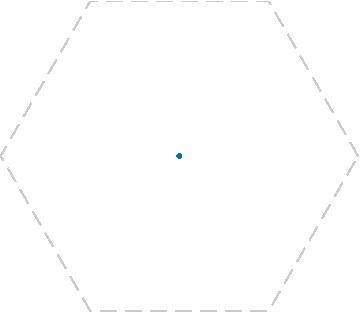
\includegraphics[width=.9\linewidth]{kuvat/6kulmio0.pdf}
        \caption{}
    \end{subfigure}%
    \begin{subfigure}[t]{.225\textwidth}
        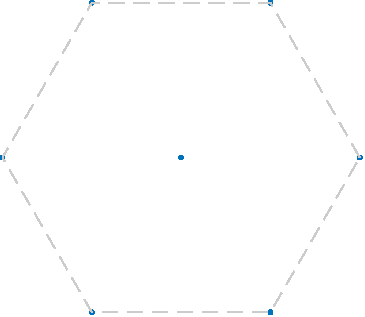
\includegraphics[width=.9\linewidth]{kuvat/6kulmio1.pdf}
        \caption{}
    \end{subfigure}%
    \begin{subfigure}[t]{.225\textwidth}
        \includegraphics[width=.9\linewidth]{kuvat/6kulmio2.pdf}
        \caption{}
    \end{subfigure}%
    \begin{subfigure}[t]{.225\textwidth}
        \includegraphics[width=.9\linewidth]{kuvat/6kulmio3.pdf}
        \caption{}
    \end{subfigure}%
    \caption{Kuusikulmion jakaminen kerroksiin. Harmaa katkoviiva kuvaa kuusikulmion kehää. Siniset pisteet ovat kuusikulmion jakavien tasasivuisten kolmioiden kärkipisteitä. Kuvassa (a) kerroksia on nolla, eli pisteitä on yksi. Kuvassa (b) on yksi kerros ja yhteensä 7 pistettä. Kuvassa (c) on kolme ja kuvassa (d) neljä kerrosta sekä vastaavasti 19 ja 37 pistettä.}
    \label{fig:6kulmio}
\end{figure}

Havaitaan, että kerrosten lukumäärän $n_k$ lisääntyessä yhdellä, olettaen $n_k>0$, pisteiden lukumäärä lisääntyy $6n_k$:lla. Siis, jos kerroksia on $n_k$ kappaletta, niin pisteitä on
\begin{equation}\label{eqn:pisteidenlkm}
    n_p=1+\sum\limits_{l=0}^{n_k}6l
\end{equation}
kappaletta. Koska funktiolle \texttt{computeHexShifts2D} syötetään pisteiden lukumäärä, tasaista asettelua varten täytyy määrittää pienin kerrosten lukumäärä $n_k$, jolle kaikki pisteet mahtuvat. Käytännössä yhtälöstä (\ref{eqn:pisteidenlkm}) täytyy ratkaista muuttuja $n_k$, joka tapahtuu aritmeettisen summan osasumman\cite{harjulehto_analyysia_2022} avulla. Osasummasta saadaan
\begin{equation*}
    n_p-1=6\frac{n_k(n_k+1)}{2},
\end{equation*}
joka on muuttujan $n_k$ toisen asteen yhtälö. Yhtälön juuret ovat
\begin{equation*}
    n_k=\frac{1}{2}\left( \pm\sqrt{4\cdot\frac{n_p - 1}{3} + 1} - 1 \right)
\end{equation*}
ja koska kerrosten lukumäärän täytyy olla epänegatiivinen, saadaan
\begin{equation*}
    n_k=\frac{1}{2}\left( \sqrt{4\cdot\frac{n_p - 1}{3} + 1} - 1 \right).
\end{equation*}
Kerrosten lukumäärän täytyy olla myös kokonaisluku, joten pyöristetään kerrosten lukumäärä kattofunktiolla ylöspäin lähimpään kokonaislukuun. Siten
\begin{equation}\label{eqn:kerrostenlkm}
    n_k=\left\lceil\frac{1}{2}\left( \sqrt{4\cdot\frac{n_p - 1}{3} + 1} - 1 \right)\right\rceil.
\end{equation}
Yhtälö (\ref{eqn:kerrostenlkm}) on toteutettu funktion \texttt{computeHexShifts2D} rivillä 10.

Riveillä 12 ja 13 asetetaan tilapäiset muuttujat kuusikulmion pisteen sijainnille. Riviltä 15 eteenpäin käydään läpi jokainen kuusikulmion kerros, jokaisen kerroksen kärki ja asetetaan tilapäisten muuttujien arvoiksi kärjen sijainti. Kerroksella $n_k$, $n_k>0$, tilapäistä muuttujaa siirretään $6n_k$ kertaa tasaisin välein ja pisteet tallennetaan vektoriin \texttt{hexShifts}. Joka lisäyksellä tarkistetaan, onko vektori \texttt{hexShifts} täynnä. Jos on, niin vektori palautetaan.

Funktion \texttt{computeSpectHexShifts} riveillä 3--9 parametrit asetetaan muuttujiin, joita käytettiin funktion kehitysvaiheessa MATLABissa. Riveillä 12--15 määritetään detektoripaneelin ulkonormaalivektori. Paneelin kulma positiiviseen $x$-akseliin nähden on laskettu rivillä 18. Riveillä 21--28 lasketaan detektorin pikselin keskipiste ja reunat detektoripaneelin $xy$-tasossa. Näitä tietoja tarvitaan siirtäessä lasketut säteet detektoripaneelin tasosta kolmiulotteiseen avaruuteen. Rivit 31--56 määrittävät kuusikulmioiden väliset etäisyydet $x$- ja $y$-suunnissa sekä säteiden päätepisteiden siirrot yhdessä kollimaattorin reiässä. Kollimaattorin reikien keskipisteet ovat laskettu riveillä 59--91 tarkalle mallille 1 ja riveillä 92--96 tehokkaalle mallille 2. Viimeinen vaihe on säteen päätepisteiden siirtojen lisääminen jokaisen kollimaattorin reiän keskipisteeseen ja koordinaatistomuunnos paneelin tasosta kolmiulotteiseen avaruuteen. Siirtojen lisääminen tapahtuu riveillä 104--107 ja koordinaatistomuunnos riveillä 114--119. Pisteet tallennetaan palautettavaan vektoriin \texttt{hexShifts}, jonka lopusta poistetaan ylimääräiset alkiot rivillä 130.

\subsection{Nelikulmainen kollimaattorin reikä}
Kuvissa \ref{fig:ray3_2D} ja \ref{fig:ray3_3D} on esitetty kolmas malli, jossa säteiden päätepisteet jakautuvat tasaisesti detektorin pikselin sisälle.

\begin{figure}[H]
    \centering
    \captionsetup{width=.9\linewidth}
    \includegraphics[width=.9\linewidth]{kuvat/malli3_2D.pdf}
    \caption{Kollimaattorin mallin 3 havainnollistus detektorin ($x$, $y$)-tasossa. Detektoripaneelin pikselit ovat rajattu punaisilla viivoilla ja detektorin havaitsemat säteet (64 kappaletta) sinisellä värillä. Detektorin pikselin koko on $(\qty{4.664}{\milli\meter})^2$.}
    \label{fig:ray3_2D}
\end{figure}
\begin{figure}[H]
    \centering
    \captionsetup{width=.9\linewidth}
    \includegraphics[width=.9\linewidth]{kuvat/malli3_3D.pdf}
    \caption{Kollimaattorin mallin 3 havainnollistus kuva-alueen transversaalitasossa. Kuva-alue on piirretty harmaalla ruudukolla ja detektorin havaitsemat säteet (64 kappaletta) sinisellä värillä. Kollimaattorin reiän pituus on \qty{32.4}{\milli\meter}, reiän halkaisija on \qty{1.4}{\milli\meter} ja reikien välinen etäisyys on \qty{0.12}{\milli\meter}. Detektorin pikselin koko on $(\qty{4.664}{\milli\meter})^2$ ja kuva-alueen yksittäisen vokselin koko on $(\qty{4.664}{\milli\meter})^{3}$.}
    \label{fig:ray3_3D}
\end{figure}

Malli on toteutettu yhdellä funktiolla \texttt{computeSpectSquareShifts}, joka on esitetty \hyperref[appendix:malli3]{liitteessä \ref*{appendix:malli3}}. Funktion rivit 1--15 ovat kuten kuusikulmaisen kollimaattorin mallissa, mutta riveillä 17--24 asetetaan pikselin koko näennäisesti suuremmaksi lähempänä kuva-aluetta. Samalla huomioidaan se, kuinka paljon säteet leviävät kuva-alueessa kollimaattorin epäideaalisuuden vuoksi. Tässä mallissa kerrosten määrä käsitellään rivillä 26 hieman eri tavalla, sillä ei-täysiä kerroksia ei ole lainkaan. Riviltä 27 eteenpäin koodin logiikka on sama kuin aiemmin: lasketaan säteiden päätepisteiden siirrot detektorin tasossa ja tehdään koordinaatistomuunnos kolmiulotteisen kuva-alueen koordinaatistoon.

\subsection{OMEGA-integraatio}
Koska käyttäjän on suunniteltu muokkaavan ainoastaan MATLAB-tiedostoja ja erityisesti pääohjelmaa, C++-funktioiden lisääminen valmiiseen ohjelmistoon vaati dataa käsittelevien funktioiden muokkaamista.

Oleellisin muutos oli sinogrammin datapisteitä vastaavien säteiden määritys. Siddonin algoritmin toteutus tarvitsee kaksi pistettä säteen virittämältä suoralta kolmiulotteisessa avaruudessa, mutta sinogrammin projektiodatasta nähdään suoraan ainoastaan havaittujen säteilytapahtumien määrä pikselikohtaisesti. Edellä esitettyjen kollimaattorin mallien mukaisten suorien määritys kuva-alueessa tarvitseekin laitteen ja erityisesti kollimaattorin dimensioita. Tarvittavat dimensiot lisättiin ohjelmiston pääohjelmaan (josta edelleen C++-koodille), jotta muillakin SPECT-laitteilla kerätystä datasta voisi rekonstruoida kuvan vain pienin muutoksin. Huomioimisen arvoista on, ettei suoran virittävää kahta pistettä voi valita mistä tahansa. Siddonin algoritmin toteutuksessa huomioidaan ainoastaan pisteiden väliin jäävän janan lävistävät kuva-alueen vokselit. Tästä johtuen toinen piste on detektoripaneelin tasossa ja toinen kuva-alueen toisella puolella usean metrin päässä. Ratkaisuun päädyttiin sen yksinkertaisuuden vuoksi, koska SPECT-laitteiden kuva-alueen enimmäishalkaisija on tyypillisesti \qty{60}{\centi\meter}\cite{cherry_single_2012}.

Varsinaiset C++:lla toteutetut kollimaattorin mallit olivat suoraviivaisia lisätä ohjelmistoon. Ohjelmistossa oli valmiina loogiset muuttujat \texttt{CT} ja \texttt{PET}, joilla voidaan määrittää kullakin kuvantamismenetelmällä ajettavat koodin osiot. Vastaavasti ohjelmistoon lisättiin muuttuja \texttt{SPECT}. Liitteissä esitetyt funktiot lisättiin lähdekoodiin sellaisenaan ja niitä kutsuttiin \texttt{SPECT}-muuttujan ehtolauseessa ennen säteiden ja vokseleiden leikkausten laskemista. Koska tässä työssä toteutetut funktiot \texttt{computeSpectHexShifts} ja \texttt{computeSpectSquareShifts} palauttavat joukon pisteitä, säteiden ja vokseleiden leikkaukset lasketaan jokaiselle parille pisteitä erikseen ja tulokset keskiarvoistetaan.

OMEGA avoimen lähdekoodin ohjelmistona on saatavissa GitHubista\footnote{\url{https://github.com/villekf/OMEGA}}. SPECT-rekonstruktio on tarkoitus sisällyttää versioon 2.0, jonka julkaisun on suunniteltu ajoittuvan vuoden 2024 lopulle.

\subsection{Projektiodatan simulointi}
Suomessa kliinisen datan tutkimuskäyttöä sääntelee niin kutsuttu toisiolaki, joka edellyttää joko luvan hakemista sosiaali- ja terveysalan tietolupaviranomaiselta Findatalta tai luvan keräämistä kuvantamisen yhteydessä potilaalta. Lupaprosessin vaatiman ajan vuoksi tässä työssä ei käytetty kliinistä dataa. Mallin kehitystä tämä ei kuitenkaan estänyt, koska mallin toimintaa voidaan testata myös simuloidulla datalla.

Ohjelmistoja emissiotomografiadatan simulointiin on kehitetty jo 1980-luvulta alkaen\cite{ljungberg_monte_1989}. Kirjallisuudessa esiintyviä, julkisesti saatavissa olevia, ohjelmistoja ovat muun muassa SIMIND\cite{ljungberg_monte_1989, taheri_monte_2017, giannone_monte_1999}, GATE (\textit{Geant4 Application for Tomographic Emission})\cite{jan_gate_2004, taheri_monte_2017}, MCNPX (\textit{Monte Carlo N-Particle Transport})\cite{taheri_monte_2017}, SIMSET\cite{giannone_monte_1999}, MCMATV3D\cite{giannone_monte_1999} ja SIMSPECT\cite{giannone_monte_1999}.

Simuloinnissa käytetyt Monte Carlo -menetelmät perustuvat satunnaisuuteen. Käytännössä tunnettuna ovat kuvattavan kohteen rakenne, materiaalit ja aktiivisuusjakauma sekä gammakameran ominaisuudet. Aktiivisuusjakauman perusteella luodaan satunnaisesti gammafotoneja sekä niille sijainti, etenemissuunta ja energia kyseessä olevan radionuklidin ominaisuuksien kaltaisesti. Jokaista fotonia seurataan sen edetessä aineessa, samalla mallintaen vuorovaikutusta satunnaisena. Vuorovaikutus mallinnetaan myös detektorissa, jolloin fotonin mahdollinen havaitseminen tallennetaan. Prosessi toistetaan miljoonia kertoja, jolloin saadaan ohjelmistolle syötettyjä parametrejä vastaavaa projektiodataa.\cite{ljungberg_monte_1989}

Tässä työssä projektiodatan simulointiin käytettiin SIMIND-ohjelmistoa (v8.0, Lundin yliopisto)\cite{ljungberg_monte_1989}, johon on sisäänrakennettuna mallinnettuja useita fantomeja (\textit{phantom}) ja radionuklideja.

Kuvantamisen fantomi on fyysinen esine (tässä tapauksessa simuloitu), jonka tarkoituksena on esimerkiksi sisältää samankaltaisia vaihteluita radioaktiivisuuden jakaumassa kuin ihmiskehossa. Fantomilla voidaan muun muassa kalibroida laitteita ja tutkia kuvan rekonstruktiota aiheuttamatta säteilyaltistusta potilaille. Fantomit ovat erityisen hyödyllisiä näissä, koska alkuperäinen aktiivisuusjakauma tunnetaan ja on siten kvantitatiivisesti verrattavissa kalibroinnin tuloksiin tai kuvan rekonstruktioon. Jäljempänä esitetyt rekonstruktiot ovat luotu simuloiduista IQ NEMA -fantomin\cite{nema2018} ja Zubal-fantomin\cite{zubal_computerized_1994} projektiodatasta.

IQ NEMA -fantomi koostuu vesisäiliöstä, jossa on kuusi radioaktiivisella nesteellä täytettyä palloa ja säiliön keskellä olevasta kiinteästä sylinteristä\cite{nema2018, mancosu_4d-pet_2009}. Pallojen halkaisijat ovat \qtylist{10;13;17;22;28;37}{\milli\meter} ja sylinterin halkaisija on \qty{51}{\milli\meter}\cite{nema2018, mancosu_4d-pet_2009}. Pallojen aktiivisuus simulaatioissa oli välillä \qtyrange{1.19}{2.38}{\mega\becquerel\per\milli\liter} ja taustan aktiivisuus oli \qty{0.0795}{\mega\becquerel\per\milli\liter}. Radioaktiivinen aine oli metastabiilia teknetiumia ja gammakvanttien energia oli \qty{140}{\kilo\electronvolt}.

Zubal-fantomi on puolestaan malli ihmiskehosta, joka on tässä tilanteessa rajattu pään alueelle. Simuloinnin kontekstissa fantomit ovat TT-kuvia, joiden jokainen pikseli on luokiteltu kuuluvaksi tiettyyn elimeen tai kudostyyppiin.\cite{zubal_computerized_1994} Jokaista elintä tai kudostyyppiä puolestaan vastaa tietty aktiivisuus, jonka perusteella määritetään simuloitujen gammafotonien määrä.

Detektorin tuikeaineen ja kollimaattorin parametrit asetettiin vastaamaan \hyperref[tbl:precedence-parametrit]{taulukossa \ref*{tbl:precedence-parametrit}} esitettyjä Precedence 6 -laitteen parametreja\cite{peters_towards_2019}. Loput kuvantamisen parametrit ovat esitetty \hyperref[tbl:simulaation_parametrit]{taulukossa \ref*{tbl:simulaation_parametrit}}. Esimerkiksi IQ NEMA -fantomin tapauksessa yhteen projektioon simuloitiin 12579273 fotonia ja havaittuja fotoneja oli yhteensä 31521520, joka vastaa noin \qty{3.9}{\percent} kokonaismäärästä.
\begin{table}[H]
    \centering
    \captionsetup{width=.9\linewidth}
    \caption{Projektiodatan simulaation parametrit}
    %\resizebox{.9\linewidth}{!}{%
        \begin{tabular}{lcc}
            \toprule
            Parametri & Arvo & \\
            \midrule
            Energiaikkuna & \qtyrange{129.5}{150.5}{\kilo\electronvolt}\\
            Projektioiden lukumäärä & 64\\
            Projektioita vastaavat kulmat & \qtyrange{0}{360}{\degree}\\
            %Simuloitujen fotonien lukumäärä & 805073472\\
            %Havaittujen fotonien lukumäärä & 31521520\\
            Kuvantamisaika per projektio & \qty{1}{\second}\\
            Projektiokuvan koko (pikseliä) & $128\cdot 128$\\
            \bottomrule
        \end{tabular}
    %}
    \label{tbl:simulaation_parametrit}
\end{table}